\documentclass[a4paper,10pt]{article}
\usepackage[T2A]{fontenc}
\usepackage[english,russian]{babel}
\usepackage[utf8]{inputenc}
\usepackage[vmargin={3cm,2cm},hmargin={2cm,2cm}]{geometry}
\usepackage{graphicx}

\usepackage{amssymb}
\usepackage{amstext}
\usepackage{amsmath}
\usepackage[warn]{mathtext}

\usepackage{indentfirst}
\usepackage{wrapfig}
\usepackage{topcapt}

\title{Список лабораторных работ}
\newcounter{LFMSHnumber}
\setcounter{LFMSHnumber}{\the \year}
\addtocounter{LFMSHnumber}{-1987}
\date{ЛФМШ-\arabic{LFMSHnumber}, август {\the \year}~г.}


\newcommand{\figRef}[1]{рис.~\ref{#1}}
\newcommand{\FigRef}[1]{Рис.~\ref{#1}}
\newcommand{\TwoLines}[2]{\begin{array}{@{}c@{}} #1 \\#2 \end{array} }
\newcommand{\Example}{\textbf{Пример: }\par}

\graphicspath{{graph/}}

\DeclareMathOperator{\Tr}{Tr}

%\newcommand{\labtitle}[5]{
%	\textbf{#2}\par
%	\textit{#1 класс}\par
%	\textbf{Цель работы:} #3\par
%	\textbf{Оборудование:} #4\par
%	\textbf{Тема:} #5
%}

\newcommand{\labtitle}[7]{
	\textbf{#2}\par
	\textit{#1 класс}~~~\textbf{#3}\par
	\textbf{Цель работы:} #4\par
	\textbf{Оборудование:} #5\par
	\textbf{Тема:} #6
}

\newcommand{\showhints}{
	\renewcommand{\labtitle}[7]{
		\textbf{##2}\par
		\textit{##1 класс}~~~\textbf{##3}\par
		\textbf{Цель работы:} ##4\par
		\textbf{Оборудование:} ##5\par
		\textbf{Тема:} ##6\par
		\textbf{Ключевые моменты:}
		\begin{itemize} ##7
		\end{itemize}
	}
}

%\showhints

\begin{document}
\maketitle
\begin{enumerate}
	\item \labtitle
		{8}
		{Определение массы твёрдого тела}
		{рчг1}
		{измерить массу продолговатого тела с помощью имеющегося оборудования.}
		{указка, гирька известной массы, линейка, нитка, стол.}
		{центр масс. Правило рычага.}
		{\item Проводим несколько экспериментов, старые отметки должны быть убраны заранее лаборантами
			\item С какой точностью определяется центр масс?
			\item Что, если палка не перпендикулярна?
		\item Что вообще такое "--- <<центр масс>>? (такая точка тела или продолжения тела, при приложении силы к которой тело не станет вращаться)}
	\item \labtitle
		{8}
		{Определение массы плоской фигуры}
		{рчг2}
		{измерить массу плоской фигуры, не используя весы.}
		{плоское тело, линейка, гирька известной массы, стол.}
		{центр масс, правило рычага}
		{\item Проводим несколько экспериментов
		\item Как найти центр гирьки? Можно вырезать кружочек и складывать его
		\item Нужно ли опускать перпендикуляры на линию края стола?
		\item Что такое <<центр масс>>?}
	\item \labtitle
		{8}
		{Определение плотности пластилина}
		{арх1}
		{определить плотность пластилина.}
		{пластилин, линейка, цилиндрический сосуд с водой.}
		{Закон Архимеда, условие плавания тел}
		{\item Почему вытесняемый телом объём $V=S\Delta h$?
		\item Откуда берётся закон Архимеда?
		\item Сначала пусть подумают сами}
	\item \labtitle
		{8}
		{Определение плотности неизвестного металла}
		{арх2}
		{найти плотность неизвестного металла и по таблице плотностей определить, какой металл был дан.}
		{цилиндрический сосуд с водой, пластиковый стаканчик, мелкие кусочки металла, линейка.}
		{Закон Архимеда, условие плавания тел}
		{\item Сначала пусть подумают сами
		\item Рассуждения про закон Архимеда те же, что и в лабе про пластилин}
	\item \labtitle
		{8}
		{Определение плотности дерева}
		{арх3}
		{определить плотность дерева.}
		{узкий цилиндрический сосуд с водой, линейка, множество деревянных палочек естественной формы.}
		{Закон Архимеда, условие плавания тел}
		{\item Палочка запускается плавать вертикально в узкий сосуд опираясь на стенки. Если длина палочки $L$, а погружено $h$, то плотность палочки примерно равна $\rho=\frac{h}{L}\rho_{\text{в}}$.
		\item Измерения $L$ и $h$ заносятся в таблицу, вычисляются плотности. Плотности наносятся на числовую ось
		\item Они должны измерить порядка 30 палочек, лучше каждую "--- два раза, переворачивая
		\item Определяется средняя плотность, определяется статистическая погрешность <<на пальцах>> и погрешность одиночного измерения. Обсуждаем, попадает ли большая часть отметок в интервал погрешности измерений относительно среднего значения?
		\item Как правильно усреднять? Только сами плотности. Что будет, если усреднять измерения до вычисления плотности?}
	\item \labtitle
		{8}
		{Определение плотности неизвестной жидкости}
		{арх4}
		{определить плотность неизвестной жидкости.}
		{цилиндрический сосуд, вода, неизвестная жидкость, линейка, пенопласт, пластилин.}
		{Закон Архимеда, условие плавания тел}
		{\item Пусть подумают сами
		\item Идея "--- делаем нечто плавающее, смотрим, сколько нужно вытеснить воды и сколько нужно вытеснить жидкости, чтобы поддерживать плавание
		\item Стандартные рассуждения про закон Архимеда}
	\item \labtitle
		{8}
		{Определение массы тяжелого груза}
		{дин1}
		{определить массу груза, исключающего непосредственное измерение.}
		{тяжелый груз, верёвка, линейка, динамометр, не позволяющий измерить массу груза непосредственным взвешиванием.}
		{второй закон Ньютона, разложение сил на составляющие}
		{\item Как они измеряют, насколько отклоняется нить? Между чем и чем меряют расстояние?
		\item Для удобства измерений линейку можно закрепить на штатив}
	\item \labtitle
		{8}
		{Исследование неидеального источника напряжения}
		{эл-б}
		{получить зависимость тока через нагрузку от напряжения на ней при различном её сопротивлении (построить нагрузочную характеристику). Объяснить полученный результат.}
		{источник постоянного тока, реостат, амперметр, вольтметр.}
		{неидеальный источник тока. КПД и мощность потерь}
		{\item Рассказать, что такое нагрузочная характеристика. Пусть попытаются нарисовать её теоретически
		\item Уяснить, что такое внутреннее сопротивление, если это плохо понятно, показать предельные точки нагрузочной характеристики
		\item В качестве источника используем Крону, можно слегка разряженную, и реостат на 100\,Ом. Ток не должен превышать 300\,мА. Можно добавить токоограничивающий резистор в 30\,Ом последовательно с реостатом, тогда ток в 300\,мА не будет превышен
		\item Черные мультиметры в режиме вольтметра и амперметра должны быть постоянно подключены к схеме.
		\item Ничего не подключаем до того, как лаборант проверит схему!
		\item Батарейка подключается к схеме через ключ. Сначала меняется сопротивление реостата, затем кратковременно включается ключ, снимаются показания и ключ отключается. Таким образом батарейка включена минимальное время и мало разряжается}
	%\item \labtitle
	%	{8}
	%	{Определение мощности человека}
	%   {}
	%	{найти работу, совершаемую при подъеме по лестнице двухэтажного корпуса бегом и шагом. Определить развиваемую при этом мощность.}
	%	{линейка, секундомер, товарищ.}
	%	{механические работа и мощность, закон сохранения энергии.}
	%   {}
	\item \labtitle
		{8, 9}
		{Определение числа $\pi$ методом Монте-Карло}
		{стат}
		{с помощью метода Монте-Карло найти приближённое значение числа $\pi$. \textit{Суть метода Монте-Карло лаборанты расскажут дополнительно.}}
		{линейка, циркуль, несколько мелких тяжелых предметов, копировальная бумага, 2 листа бумаги.}
		{случайные события, вероятность.}
		{\item Основная идея "--- при помощи физического процесса мы генерируем равномерно распределенные точки на листе бумаги. Кладём в ящик лист, накрываем копировальной бумагой, закрепляем, насыпаем дробь и трясем. Варианты исполнения могут быть разные. Строим на листе бумаги круг и квадрат и по отношению количества точек определяем отношение площадей, откуда число $\pi$.
		\item Какие преимущества метод Монте-Карло имеет перед тем, чтобы просто построить круг на миллиметровке и посчитать площадь. }
	\item \labtitle
		{8, 9}
		{Измерение длины нити накаливания лампочки}
		{опт1}
		{измерить размеры нити накаливания лампочки, используя линзы для переноса изображения.}
		{лампочка с источником питания, собирающая линза, оптический стол.}
		{геометрическая оптика.}
		{\item Идея "--- построить увеличенное изображение нити накаливания лампочки на экране-миллиметровке, зарисовать, затем измерить
		\item Вспоминаем геометрическую оптику. Как строятся изображения в тонких линзах. Действительное, мнимое, перевернутое, прямое, увеличенное, уменьшенное...
		\item (Мой любимый вопрос на понимание оптики) Как работает лупа?}
	%\item \labtitle
	%	{8}
	%	{Закон Джоуля-Ленца}
	%   {}
	%	{экспериментально проверить справедливость закона Джоуля-Ленца.}
	%	{вода, нагревательная спираль, регулируемый источник напряжения, термометр, секундомер.}
	%	{электрическая мощность, закон Джоуля-Ленца.}
	%   {}
	\item \labtitle
		{8, 9}
		{Измерение расстояний на местности}
		{ул1}
		{измерить на местности расстояние до недоступного объекта.}
		{измерительная лента (рулетка), компас или транспортир.}
		{метод триангуляции.}
		{\item Некоторая вытянутая территория "--- это <<пол>>. Остальное "--- лава. Нужно определить расстояние от одного из концов пола до объекта в <<лаве>>. Например, южное крыльцо лаб "--- <<пол>>, а всё остальное пространство лагеря "--- <<лава>>. А определить нужно расстояние, скажем, до ногомойки.
        \item Суть работы "--- решение треугольника. На <<полу>> располагаются две вершины (одна сторона). Третья вершина "--- недоступный объект. При помощи транспортира или компаса (через азимут) определяются углы между сторонами, при помощи длинной рулетки определяется длина стороны на <<полу>>.}
	\item \labtitle
		{8, 9}
		{Исследование мощности лампочки}
		{эл-л}
		{исследовать зависимость мощности, потребляемой лампой накаливания, от поданного на неё напряжения.}
		{регулируемый источник тока, лампа накаливания, соединительные провода, два вольтметра, известное сопротивление.}
		{закон Ома. Электрическая мощность.}
		{\item По закону Джоуля-Ленца, $P=\frac{U^2}{R}$. На первый взгляд, зависимость должна быть квадратичной, и это нужно проверить, построив $P(U^2)$ (пусть попробуют сами догадаться, что график нужно строить в таких осях). Зависимость не будет чисто квадратичной, поскольку температура нити накаливания сильно меняется, а сопротивление зависит от температуры
        \item Пусть получат сами более точную форму зависимости из следующих соображений: сопротивление металла пропорционально абсолютной температуре $R \propto T$. Практически вся подводимая мощность тратится на излучение, но по закону Стефана-Больцмана $P \propto T^4$. Если учесть это в законе Джоуля-Ленца $P=\frac{U^2}{R}$, несложно вывести, что $P \propto U^\frac{8}{5}$
        \item Чтобы по экспериментальным точкам определить значение показателя степени $U$, можно построить $P(U)$ в двойных логарифмических осях, то есть $ln(P)[ln(U)]$. В таких осях степенная зависимость превращается в линейную, а угол наклона прямой соответствует показателю степени
        \item Помимо точек по напряжению, в которых лампочка светится, следует промерить точки до момента, когда нить становится заметно красной}
	\item \labtitle
		{8, 9, 10}
		{Определение фокусного расстояния линз}
		{опт2}
		{определить фокусное расстояние собирающей и рассеивающей линз.}
		{лампочка с источником питания, собирающая и рассеивающие линзы, белый лист картона.}
		{геометрическая оптика.}
		{\item Вспоминаем геометрическую оптику. Как строятся изображения в тонких линзах. Действительное, мнимое, перевернутое... Формула тонкой линзы! Концепция того, что когда у нас несколько линз, следующая видит изображение предыдущей
		\item Как в целом устроена логика лабы: сначала строим в собирающей линзе изображение лампочки, измеряем расстояния до лампочки и изображения, по формуле тонкой линзы вычисляем её фокусное расстояние. С рассеивающей линзой проблема в том, что она всегда создаёт мнимое изображение, расстояние до него не измерить прямым образом. Поэтому собираем систему: ставим рассеивающую линзу, затем собирающей переводим мнимое изображение в действительное. Зная фокусное расстояние собирающей, восстанавливаем расположение промежуточного мнимого изображения
		\item Есть альтернативный способ найти фокусное расстояние собирающей линзы: построить на экране изображение <<бесконечно удалённого>> объекта, например облаков или крон деревьев. Изображение будет примерно в фокусе
		\item Про погрешности: линза не тонкая. Как правильно измерить расстояние до толстой линзы "--- непонятно, поэтому разумно выбрать толщину линзы за погрешность
		\item А как работает лупа?}
	\item \labtitle
		{9}
		{Исследование периода колебаний пружинного маятника}
		{клб1}
		{Исследовать зависимость периода колебаний пружинного маятника от массы груза. Найти значение периода теоретически, измерив коэффициент упругости отдельно.}
		{Набор грузов известной массы, штатив с лапками для закрепления пружин, линейка, секундомер.}
		{закон Гука. Колебания.}
		{\item}
	\item \labtitle
		{9}
		{Определение коэффициента трения}
		{дин1}
		{Определить коэффициент трения между деревом и деревом; между деревом и материалом, покрывающим пол.}
		{Штатив, две ученические линейки, угольник.}
		{сухое трение.}
		{\item}
	\item \labtitle
		{9}
		{Определение модуля Юнга}
		{упр1}
		{Определить модуль Юнга резинового жгута при деформации растяжения.}
		{Банковские резинки, штангенциркуль или микрометр, линейка, набор грузов известной массы, штатив.}
		{закон Гука. Модуль Юнга.}
		{\item Проводим минимум два эксперимента: банковские резинки разрезаны и связаны друг с другом в длинную одинарную резинку и резинки без разрезания соединены в двойную цепочку}
	\item \labtitle
		{9}
		{Определение доли вращательной энергии}
		{двд1}
		{Определить долю вращательной энергии при скатывании тела по наклонной плоскости в зависимости от угла наклона желоба.}
		{Штатив, желоб, линейка, шарики разных масс, весы, секундомер.}
		{закон сохранения энергии. Вращательное движение.}
		{\item}
	\item \labtitle
		{9}
		{Определение жесткости последовательно и параллельно соединенных пружин}
		{упр2}
		{Определить жесткость параллельно и последовательно соединенных пружин экспериментально и теоретически}
		{Две пружины неизвестной жесткости, штатив с лапками, линейка, набор грузов известной массы.}
		{механика. Закон Гука.}
		{\item}
	\item \labtitle
		{9, 10}
		{Маятник Максвелла}
		{двд2}
		{Определить момент инерции маятника Максвелла и скорость потерь энергии при его колебаниях.}
		{Штатив, секундомер, линейка, штангенциркуль, маятник Максвелла.}
		{колебания. Вращательное движение.}
		{\item Лаба требует хотя бы поверхностного понимания момента инерции. Про момент инерции можно конечно рассказывать фундаментально, умножив второй закон Ньютона справа на радиус-вектор, кратко рассказав вывод ОУДВД и потом энергии вращения. Но можно зайти с более простой стороны рассказать про него сразу со стороны энергии. Посмотрим, какая кинетическая энергия будет у тела, которое движется и ещё вращается. Понятно, что это не просто $\frac{mV^2}{2}$, потому что некоторые части тела двигаются быстрее $V$, а некоторые "--- медленнее. Можно доказать, что с точки зрения энергии поступательное движение и вращение относительно центра масс "--- независимы, то есть энергии можно посчитать отдельно и сложить. Но доказывать это имеет смысл только тем, кто поумнее. Остальным можно просто сообщить, как факт. Теперь, посмотрим, как устроена энергия тела, вращающегося с угловой скоростью $\omega$. Рассмотрим произвольный маленький кусочек тела на расстоянии $r_i$ от центра вращения (который совпадает с центром масс). Энергия его движения будет $\Delta E_i = \frac{\Delta m_i V_i^2}{2} = \frac{\Delta m_i r_i^2 \omega^2}{2}$. Если мы просуммируем по всем таким маленьким кусочкам энергию, то получим некую величину $E=\frac{I\omega^2}{2}$, причём по размерности $[I] = \text{кг}\cdot\text{м}^2$, а значит его можно представить в виде $I=\alpha mR^2$ для тела, которое имеет только один линейный размер $R$. Разные симметричные тела будут отличаться значением коэффициента $\alpha$.
        \item Для маятника Максвелла, который опускается из верхней точки вниз, можно записать ЗСЭ:
        \begin{equation*}
            mgh = \frac{mV^2}{2} + \frac{I\omega^2}{2} \quad \implies \quad 2gh = V^2 + \frac{\alpha R^2}{r^2}V^2 \quad \implies \quad \alpha = \frac{r^2}{V^2R^2}(2gh - V^2),
        \end{equation*}
        где $R$ "--- радиус маятника максвелла, а $r$ "--- радиус его оси. Таким образом мы можем найти коэффициент $\alpha$ в составе момента инерции, что и будет одной из целей работы
        \item Второе задание "--- построить график доли потерянной энергии от амплитуды или от периода маятника Максвелла. Смысл в том, что при низкой амплитуде имеет место более упругое растяжение нити в нижней точке и доля потерянной энергии должна быть меньше
        }
	\item \labtitle
		{9, 10}
		{Определение отношения сопротивлений}
		{эл-с}
		{Определить отношение сопротивлений двух резисторов.}
		{Источник питания, близкий к идеальному, вольтметр, два резистора сопротивлением порядка единиц МОм, соединительные провода.}
		{электричество. Закон Ома.}
		{\item В лабе используются мегаомные резисторы и черные простенькие мультиметры. Это принципиально, потому что внутренние сопротивления вольтметров должны быть порядка сопротивлений резисторов, в этом суть лабы
        \item Самое очевидное решение задачи "--- соединить последовательно резисторы $R_1$ и $R_2$, подключить их к источнику и померить напряжение на каждом из них. Но если просто поделить напряжения $U_{R1}$ и $U_{R2}$ друг на друга, результат получится неправильный, поскольку резисторы будут шунтироваться внутренним сопротивлением вольтметра. Можно поступить двумя способами: либо решить задачу с учётом внутреннего сопротивления вольтметра, либо пойти на хитрость. Можно подключить к источнику резистор с вольтметром \textit{последовательно}, и найти отношение сопротивлений каждого из резисторов к внутреннему сопротивлению вольтметра}
	\item \labtitle
		{9, 10}
		{Определение ёмкости конденсатора}
		{эл-к}
		{Определить емкость конденсатора про помощи баллистического гальванометра. \textit{Суть метода расскажут лаборанты.}}
		{Набор конденсаторов известной емкости, конденсатор неизвестной емкости, микроамперметр, источник напряжения, переключатель.}
		{Электрическая ёмкость, баллистический гальванометр.}
		{\item Разбираемся, что такое электрическая ёмкость и конденсатор. Можно рассказать, как конденсатор заряжается от источника через резистор и как разряжается через резистор. Нарисовать графики напряжения от времени. Это поможет привыкнуть к концепции конденсатора

        \item Объясняем баллистический гальванометр. Основная идея: стрелочный микроамперметр "--- это стрелка, которую пружинка возвращает в 0. Внутри прибора находится электромагнит (катушка с проводами), который притягивает стрелку, отклоняя её, сопротивляясь пружине. Сила, отклоняющая стрелку $F\propto B\propto I$. Если ток протекает кратковременно, то импульс стрелки $p = F\Delta t \propto I\Delta t = \Delta q$. Поскольку стрелка возвращается в 0 пружиной, можно сказать, что $\frac{mV_0^2}{2} = \frac{k\Delta x^2}{2}$, то есть расстояние, на которое отклонится стрелка, выраженное в числе делений $\Delta N \propto \Delta q$
        \begin{figure}[h]
            \centering
            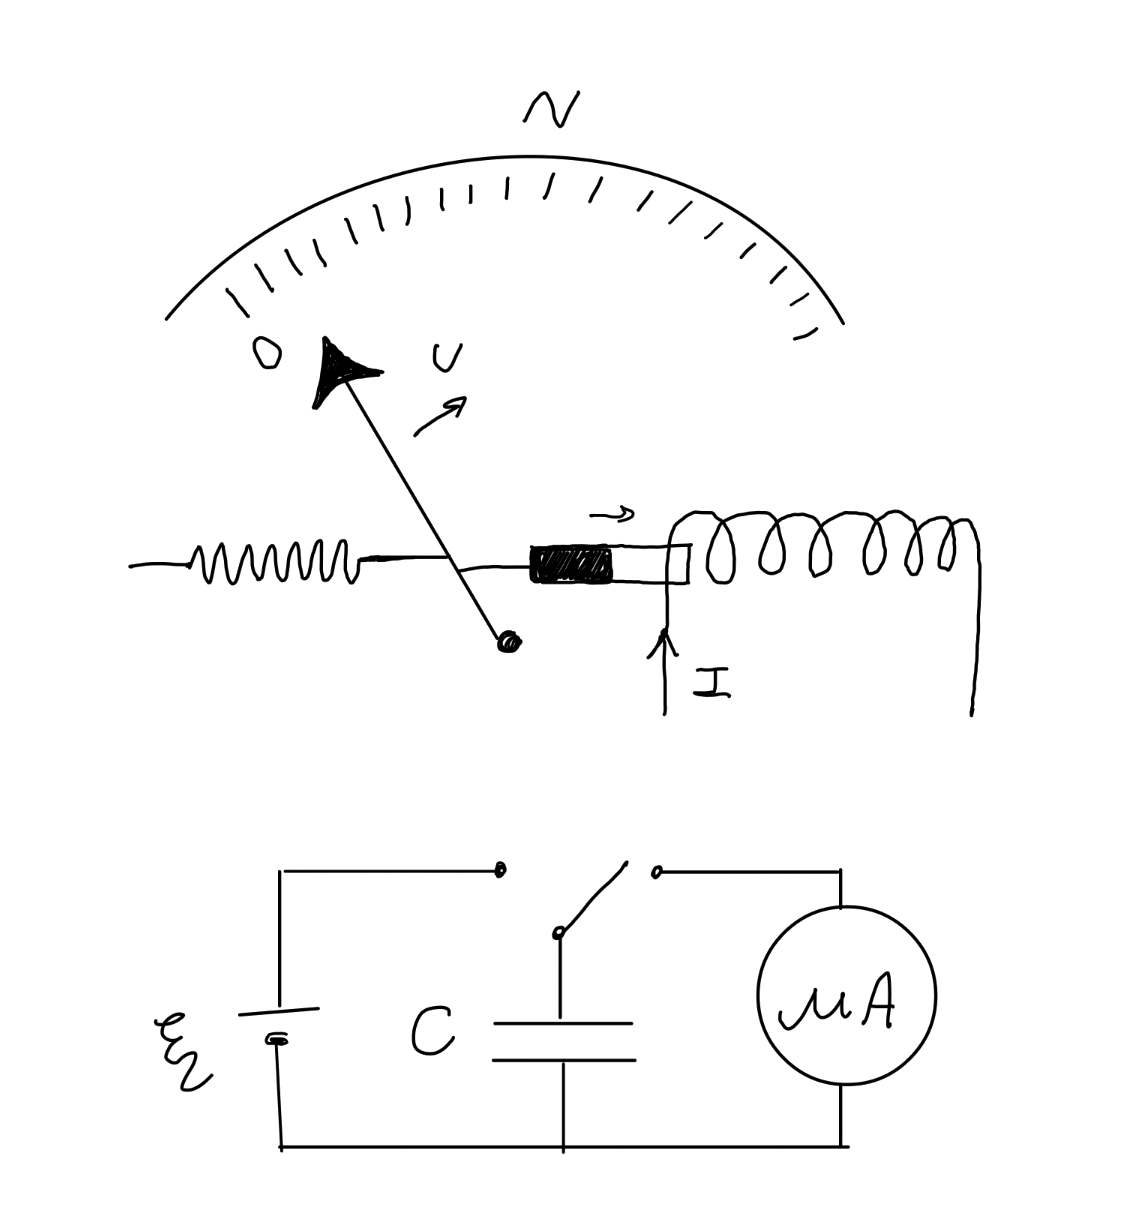
\includegraphics[width=0.5\textwidth]{ballistic-galva.png}
            \caption{Условное строение амперметра и схема, которую нужно собрать}
            \label{fig:ballistic}
        \end{figure}
        \item Рисуем схему. Заряд на конденсаторе $q = CU$. Напряжение источника мы не меняем. Когда он разряжается через микроамперметр, отскок стрелки пропорционален заряду, который пропорционален ёмкости. Значит, количество делений, на которое отклонилась стрелка $\Delta N = \alpha C$. Собираем схему с известными конденсаторами, находим $\alpha$. Собираем схему с конденсатором неизвестной ёмкости, и вычисляем его ёмкость
        \item Питание к схеме подключается \textbf{только после} её проверки лаборантом! Если микроамперметр окажется подключенным к источнику, он мгновенно перегорит. Использование ключа в схеме обязательно!}
	\item \labtitle
		{9, 10}
		{Определение скорости звука}
		{осц-зв}
		{определить скорость звука в воздухе и в дереве по задержке сигнала при распространении в среде}
		{осциллограф, два микрофона, линейка.}
		{колебания, волны.}
		{\item В этой работе нужно рассказать про то, как устроен динамик и микрофон. Основная идея "--- диффузор соединён с катушкой с проводом, который находится в магнитном поле. Если подавать переменное напряжение, то катушка начинает притягиваться к магниту и отталкиваться от магнита и диффузор будет колебать воздух. В обратную сторону (как микрофон) это тоже работает: воздух колеблет диффузор, он перемещает катушку в магнитном поле и в соответствии с законом электромагнитной индукции Фарадея в катушке возникает ЭДС, которую мы можем посмотреть на осциллографе
        \item Измерение скорости звука в дереве проводится на лавке, сидение которой сделано из цельных досок. В результате измерений всегда получается скорость существенно ниже табличной, которая для сосны вдоль волокон составляет 3600\,м/с. Лучшее объяснение эффекта, которое мы придумали "--- что большая часть звуковых <<лучей>> проходит не напрямую вдоль доски, а <<зигзагом>>, отражаясь от её границ. Таким образом путь значительно увеличивается.
        \item Допвопрос. \textit{Только для пионеров, посещающих душ.} Когда вы ходите с друзьями в лагерный душ, то начиная с некоторого расстояния очень трудно понимать, что говорит другой человек. Даже если вода выключена. Вне зависимости от того, как громко произносится фраза. Объясните это явление. \textit{Ответ:} звук, который мы произносим, распространяется во все стороны. Некоторая его часть идёт напрямую в уши слушателям, некоторая "--- отражается от стен один или несколько раз и приходит с задержкой. Когда люди стоят близко, то путь звука без отражений значительно короче, чем отраженного, и его относительная громкость выше. Он перебивает отражения и слышно хорошо. Начиная с некоторого расстояния соотношение отраженного и <<прямого>> сигнала становится больше, и из-за наложения звука ничего не понятно}
	\item \labtitle
		{10}
		{Определение атмосферного давления}
		{вод1}
		{Определить атмосферное давление с помощью имеющегося оборудования.}
		{Резиновый шланг, воронка, рулетка, штатив, линейка.}
		{атмосферное давление. Давление столба жидкости. Газовые законы.}
		{\item}
	\item \labtitle
		{10}
		{Определение площади комнаты}
		{кол2}
		{Определить площадь комнаты с помощью математического маятника.}
		{штатив, секундомер, груз, нить.}
		{колебания. Математический маятник.}
		{\item}
	%\item \labtitle
	%	{10}
	%	{Жесткость пружины}
	%   {}
	%	{Экспериментально проверить зависимость периода колебания пружинного маятника от массы груза и жёсткости пружины.}
	%	{штатив, набор грузов, пружины, секундомер, линейка.}
	%	{колебания. Пружинный маятник.}
	%   {}
%	\item \labtitle
%		{10}
%		{Определение ЭДС и внутреннего сопротивления источника}
%       {}
%		{вычислить ЭДС и внутреннее сопротивление источника тока по результатам измерений силы тока в цепи и напряжения на участке цепи.}
%		{источник постоянного тока, вольтметр, амперметр, два резистора неизвестного сопротивления, соединительные провода.}
%		{закон Ома. Неидеальный источник ЭДС.}
%       {}
	\item \labtitle
		{10}
		{Вольт-амперная характеристика нелинейного элемента}
		{осц-вах}
		{построить вольт-амперную характеристику нелинейного элемента \textit{на экране осциллографа.}}
		{исследуемый нелинейный элемент, резистор известного сопротивления, источник переменного напряжения, осциллограф.}
		{вольт-амперная характеристика. }
		{\item}
	\item \labtitle
		{10}
		{Измерение постоянной Планка $\hbar$}
		{плнк}
		{изучить явление фотоэффекта. Построить зависимость фототока от напряжения на аноде, построить зависимость запирающего напряжения от частоты света. Определить значение постоянной Планка.}
		{источник белого света, набор светофильтров, фотоэлемент, установка для измерения фототока при различных анодных напряжениях}
		{основы квантовой теории света. Фотоэффект}
		{\item}
	\item \labtitle
		{9, 10}
		{Определение доли энергии, рассеиваемой при соударении}
		{осц-эн}
		{определить долю энергии, рассеиваемой шариком при отскоке от различных поверхностей}
		{шарик, микрофон, осциллограф}
		{закон сохранения энергии. Равноускоренное движение.}
		{\item Мы роняем шарик на стол. Он отскакивает от стола, теряя часть энергии. Если он в воздухе находится время $\Delta t$, значит его скорость в нижней точке $V=\frac{gt}{2}$, а энергия "--- $E=\frac{mg^2\Delta t^2}{8} \propto \Delta t^2$
		\item При помощи осциллографа определяем моменты, в которые шарик соприкасался со столом. Определяем времена нахождения шарика в воздухе и вычисляем долю энергии, которую он теряет при соударении со столом.
		\item Строим график доли потерянной энергии от времени нахождения в воздухе, о нём можно поговорить. Основная идея "--- при большой амплитуде удар сильный и неупругий, а при маленькой "--- упругий и энергий почти не теряется
		\item Рассказать про микрофон и динамик как в лабе про скорость звука
		\item Рассказать про работу с осциллографом, про синхронизацию и курсоры}
	\item \labtitle
		{10}
		{Изучение распространения электромагнитных волн СВЧ диапазона}
		{свч}
		{определить длину волны сверхвысокочастотного (СВЧ) излучателя, определить диэлектрическую проницаемость парафина.}
		{СВЧ-излучатель, осциллограф, активный и пассивные СВЧ-детекторы}
		{электромагнитные волны.}
		{\item Рассказываем про уравнение плоской скалярной волны $U(x, t) = A \cos(\omega t - kx)$. Выясняем, что такая волна бежит в положительную сторону по $x$.
		\item Рассказываем про электромагнитные волны, вектора $\vec E$ и $\vec B$, поляризацию. Рассказываем, что ЭМВ бывают разной частоты, разницу между радиоволной и светом.
		\item Как принимаются радиоволны. Как волна воздействует на антенну. Как сделать детектор? (поставить диод в разрез антенны)
		\item Что будет, если навстречу летят две плоские волны (будет стоячая волна). А что, если разной амплитуды?
		\item Переходим к установке. Источник излучает модулированную прямоугольником порядка 1\,кГц волну. Показываем поляризацию, отражение от пластины, стоячую волну
		\item Если хватает времени, устанавливаем парафиновую призму и смотрим, как она преломляет, находим коэффициент преломления
		\item Обеспечиваем передоз знаниями}
\end{enumerate}
\end{document}

